\subsection{Case study overview}
We focus on the San Francisco Bay Area, a seismically-active region, to illustrate our approach (Figure~\ref{fig:equity_study_area}). The area follows a polycentric metropolitan form, with San Francisco as the primary center and other jobs  concentrated in suburban centers, such as Silicon Valley~\cite{cervero_polycentrism_1997}. The region has a wide array of trip patterns for mandatory and non-mandatory trips. Furthermore, trip times and routes vary greatly depending on travel preferences and workplace locations~\cite{cervero_polycentrism_1997}. Thus,  we might expect noticeable disparities between households in the risk of travel time delays due to earthquakes. 

\begin{figure}
\centering
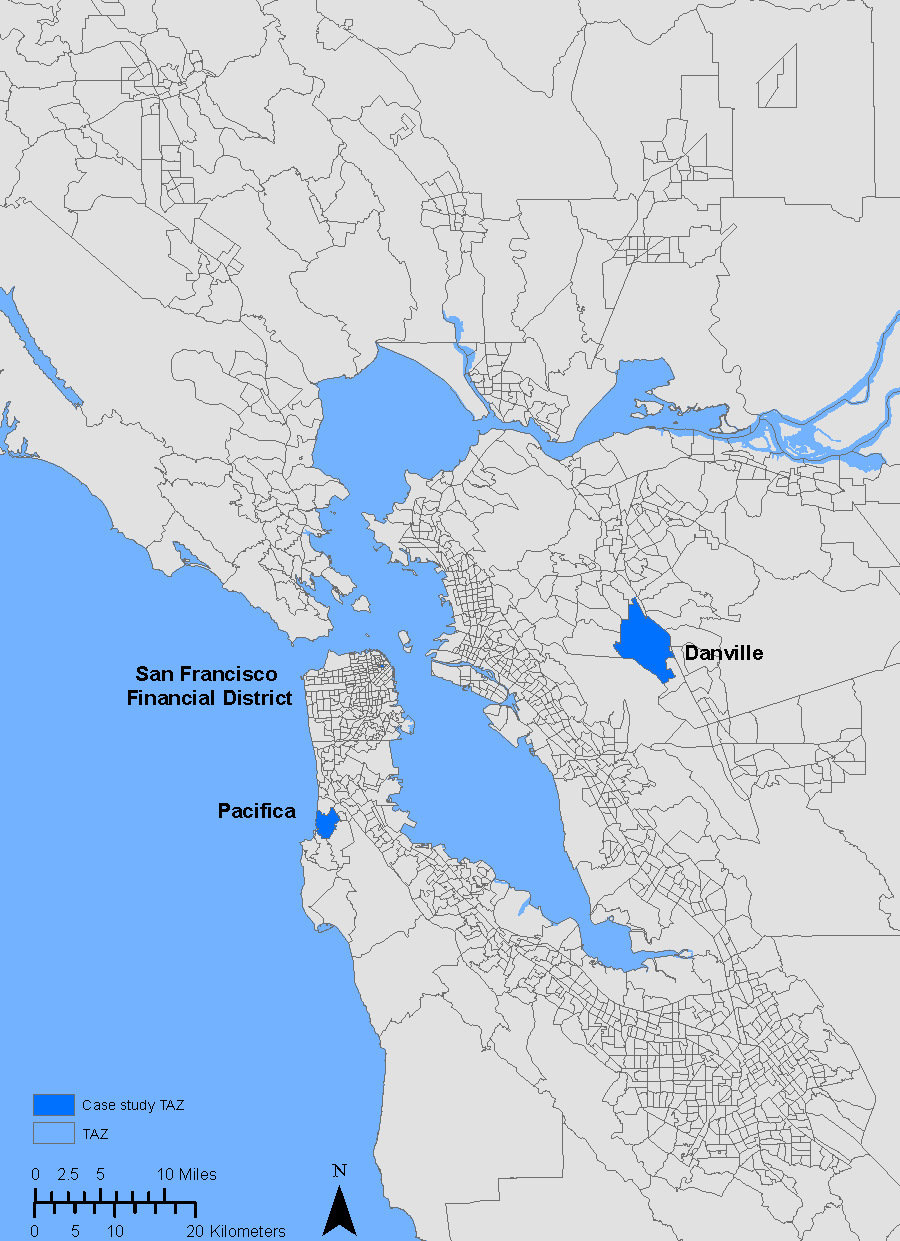
\includegraphics[width=6in]{FIGS/equity_case.pdf} 
\caption{Study area: San Francisco Bay Area, CA with specific travel analysis zones (TAZs) used in the case study marked in blue.}
\label{fig:equity_study_area}
\end{figure}

This analysis considers the complex web of roads and transit networks of the case study area. The roads are modeled by a directed graph $G = (V, E)$, where $V$ is a finite set of vertices representing intersections, and the set $E$, whose elements are edges representing road links, is a binary relation on $V$. In this model, $(|V|, |E|)$ = (11,921, 32,858) including centroidal links and $(|V|, |E|)$ = (9,635, 24,404) without. Centroidal links do not correspond to particular physical roads but instead capture more subtle travel flows, such as  from outside the study area or the flow of people to and from some minor local roads. We also model 43 transit networks, as detailed in Miller 2014~\cite{miller_seismic_2014}.

We  model damage to a set of 1743 highway bridges impacting the road and some transit networks, with data provided by the California Department of Transportation (Caltrans), and 1409 structures impacting the rapid transit network, BART, with data provided by that agency. We refer readers to Miller 2014~\cite{miller_seismic_2014} for more details about matching these structures, hereafter called components, to the relevant road and transit networks.


\begin{sidewaysfigure}
\centering
\includegraphics[width=\textwidth]{../FIGS/Mahalia_four_pannels204v5.pdf} %methods_Mahalia_four_pannels204v3.png} 
\caption{Illustration of the risk framework for one earthquake event including a) One-second spectral acceleration  (ground-motion intensity) map with earthquake rupture, b) bridge (component) damage map, c) map of travel time increase (network-performance measure) values, and d) map of accessibility values averaged over all market segments by travel analysis zone (TAZ). There are 1454 TAZs.}
\label{fig:four_steps}\end{sidewaysfigure}

\subsection{Ground-motion intensity maps}
\subsubsection{Theory}
We now describe how to produce a set of maps with ground-motion intensity realizations at each location of interest in a region and corresponding occurrence rates that reasonably capture the joint distribution of the ground-motion intensity. First, we generate $Q$ earthquake scenarios from a seismic source model. The seismic source model specifies the rates at which earthquakes of specified magnitudes, locations, and faulting types will occur. This set of earthquake scenarios is comparable to a stochastic event catalogue in the insurance industry.

Second, for each earthquake scenario in the seismic source model, we use an empirical ground-motion prediction equation (GMPE)~\cite[e.g.,][]{boore_ground-motion_2008,abrahamson_summary_2008,chiou_nga_2008,campbell_nga_2008} to model $Y$, the resulting intensity measure at each location of interest~\cite[e.g.,][]{campbell_strong_1985,baker_which_2006,foulser-piggott_predictive_2012}. %e.g., Foulser-Piggott and Stafford 2011). The GMPE predicts the mean of the log ground-motion intensity, $\overline{\ln Y (M_q, R_{iq}, V_{s30,i}, \ldots) }$ and ground-motion intensity within- and between-event residual standard deviations, which are denoted by \gls{sigma}$_{iq}$ and \gls{tau}$_q$ respectively, for the $i^{th}$ site where $i = 1, \ldots, $\gls{n} in the $q^{th}$ earthquake scenario where \gls{q}$=1, \ldots, $\gls{Q}, $M_q$ is the moment magnitude of the $q^{th}$ scenario, $R_{iq}$ is the closest horizontal distance from the surface projection of the fault plane to location $i$, and \gls{V_{s30,i}} is the average shear wave velocity down to 30$m$ at the $i^{th}$ location. 

Then, for each of the $Q$ earthquake scenarios, we sample $b$ realizations of the spatially-correlated ground-motion intensity residual terms. Readers are referred to \cite{han_probabilistic_2012} for a survey of sampling methods.  Once residuals are sampled, the total log ground-motion intensity ($Y$) is computed as 

\begin{equation}
\ln Y_{ij} = \overline{\ln Y (M_j, R_{ij}, V_{s30,i}, \ldots) }+ \sigma_{ij} \epsilon_{ij} + \tau_j \eta_j
\label{eq:GMPEmet}
\end{equation}
where $j$ is the ground-motion intensity map index ($j = 1, \ldots, m$ where $m = Q \times b$), $\epsilon_{ij}$ is the normalized within-event residual in $\ln Y$ representing location-to-location variability and $\eta_j$ is the normalized between-event residual in $\ln Y$ and the other parameters are defined above. Both $\epsilon_{ij}$ and $\eta_j$ are normal random variables with zero mean and unit standard deviation. The vector of $\epsilon_{ij}$ can be modeled by a spatially-correlated multivariate normal distribution~\cite[e.g.,][]{jayaram_correlation_2009} %Boore et al. 2003; Wang and Takada 2005; Goda and Hong 2008; Jayaram and Baker 2009 
and the $eta_j$ by a standard univariate normal distribution. 

The result is a set of $m$ ground-motion intensity maps (e.g., Figure~\ref{fig:four_steps}{(a)}). Since we simulate an equal number ($b$) of ground-motion intensity maps per earthquake scenario, the annual rate of occurrence for the $j^{th}$ ground-motion intensity map is the original rate of occurrence of the earthquake scenario, divided by $b$. We denote the final result as $w_j$.  

\subsubsection{Implementation}
To generate a stochastic catalog of ground-motion intensity maps, we use the OpenSHA Event Set Calculator~\cite{field_opensha:_2003}. This software outputs the mean, $\overline{\ln Y_{ij}}$, and standard deviation values, $\sigma_{ij}$ and $\tau_j$, for all locations of interest for a specified seismic source model and ground-motion prediction equation. The intensity measure is the 5\%-damped pseudo absolute  spectral acceleration ($Sa$) at a period $T=1s$, which is the required input to the fragility functions below. This spectral acceleration value represents the maximum acceleration over time  that a linear oscillator with 5\% damping and a period of 1 second will experience from a given ground motion. We calculate these values at each component location (bridges and other structures). Using one ground-motion intensity measure per component is a common simplification of the time-varying acceleration dynamics~\cite[e.g.,][]{shinozuka_effect_2003,jayaram_efficient_2010} that may have lower errors for compact components with a natural period near 1 second as opposed to long-span bridges~\cite{konakli_simulation_2012}.
%In other words, we follow the standard practice of using one ground-motion intensity measure per component, which is a simplification of the true dynamics involving more dependence on the acceleration time histories, spatial differences in acceleration for a component (particularly long-span bridges), and 
We use the UCERF2 seismic source model~\cite{field_uniform_2009}, Wald and Allen topographic slope model for the the shear wave velocity $V_{s30,i}$~\cite{wald_topographic_2007}, and the Boore and Atkinson \cite{boore_ground-motion_2008} ground-motion prediction equation.   Using this seismic source model, which is then discretized into a list of faults and a stratified list of magnitudes and rupture locations for each, we obtain a set of 2110 earthquake events on all active faults, each with an annual occurrence rate greater than or equal to $10^{-5}$ . We simulate the sets of maps by combining the mean terms from the Event Set Calculator and spatially-correlated residual terms of the ground-motion intensity  (using~\cite{jayaram_correlation_2009}) according to the basic ground-motion model, Equation~\ref{eq:GMPEmet}. 


\subsection{Damage maps}
\subsubsection{Theory}
Calculating network performance risk requires assessing the structural damage of relevant components after future earthquakes. The link between ground-motion intensity and structural damage is often provided by fragility functions. Fragility functions express $P(DS_i \geq ds_{\varsigma} | Y_{ij} = y)$. We assume one component, such as a bridge, per site location, so we will identify both components and site locations via the index $i$. Using that notation, $DS_i$ is a discrete random variable whose value represents the damage state for the $i^{th}$ component and $ds$ is a damage state threshold of interest. The damage state is conditioned on a realization, $y$, of the random variable $Y_{ij}$, the ground-motion intensity at the $i^{th}$ site and $j^{th}$ ground-motion intensity map. Researchers have calibrated fragility functions using historical post-earthquake data~\cite[e.g.,][]{basoz_enhancement_1999}, experimental and analytical results~\cite[e.g.,][]{ramanathan_analytical_2010}, hybrid approaches, and expert opinion. It is possible to sample the damage states from  a joint distribution that includes correlation, such as due to similarities in design or construction practices~\cite[e.g.,][]{lee_uncertainty_2007,baker_introducing_2008}. 

By sampling a damage state for each component, with probabilities obtained from the fragility functions given the ground-motion intensity, we produce a damage map (e.g., Figure~\ref{fig:four_steps}{(b)}). The damage map has a realization of the damage state of each relevant component. This sampling process can be repeated multiple times to simulate multiple damage maps per ground-motion intensity map. For example, if equal numbers of damage maps are sampled per ground-motion intensity map ($c$ damage maps per ground-motion intensity map), the weight of the $j'^{th}$ damage map should be adjusted accordingly to $w_{j'}$, where $w_{j'} = \frac{w_j}{c}$, and $j' = 1, \ldots, J$. 

%These damage maps are directly mapped to the functionality of elements of the network. 
\emph{Functional percentage} relationships link the component damage to the functionality of network elements.  For example, in a road network, when a bridge collapses, the traffic flow capacity of the road it carries and it crosses can be modeled as reduced to zero. These relationships are often derived from a combination of observation and expert opinion, often due to data scarcity~\cite{werner_redars_2006}. Furthermore, the relationships are typically deterministic for a certain component damage state and restoration time~\cite{werner_redars_2006}. Thus, in this paper, each damage map corresponds to a functionality state for every element of the network.

\subsubsection{Implementation}
\paragraph{Component damage}


%We do not include other types of network component failures such as liquefaction in this study.

We use fragility functions of the following form to provide the link between ground-motion shaking and component damage:
\begin{equation}
%$P(DS \geq ds_s | Y = y_{ij}, i)$
P(DS_i \geq ds_\varsigma |Y_{ij} = y) = \Phi \left( \frac{\ln y - \lambda_{\varsigma, i}}{\xi_{\varsigma,i}} \right),
\label{eq:dsfull}
\end{equation}
where $\Phi$ is the standard normal cumulative distribution function, $\lambda_{\varsigma,i}$ and $\xi_{\varsigma,i}$ are respectively the mean and standard deviation of the $\ln Y_{ij}$ value necessary to cause the $\varsigma^{th}$ damage state to occur or be exceeded for the $i^{th}$ component, and the other variables are defined above. By using the previous equation and the inverse method, we can sample realizations of component damage states for a given ground-motion intensity.
%
%
%where $DS_i$ is a discrete random variable, whose value represents the damage state, $s$, for each bridge index $i$. $\Phi$ is the standard normal cumulative distribution function and $\lambda_{s,i}$ and $\xi$ are respectively the mean and standard deviation of the $\ln Y$ value necessary to cause the $s^{th}$ damage state to occur or be exceeded. $y_{i,j}$ is the spectral acceleration value that the bridge experiences for the $j^{th}$ ground-motion intensity map. 

The California Department of Transportation (Caltrans) provided the fragility function values $\lambda_{\varsigma,i}$ and $\xi_{\varsigma,i}$ used in this study for the highway components in summer 2012, which was last updated in 2007 and includes various retrofitted bridges~\cite{caltrans_caltrans_2013}. The $\lambda_{\varsigma,i}$ values are based on component characteristics including number of spans and age as detailed in \cite{basoz_enhancement_1999}. The $\xi_{\varsigma,i}$ values are given as a constant. The BART seismic safety group provided the  fragility function values $\lambda_{\varsigma,i}$ and $\xi_{\varsigma,i}$ used in this study for the BART-related components for the state of the network in summer 2012. At that time, data was available for the aerial structures shown in Figure~\ref{fig:bart}. These correspond to the safety performance goals under the recent retrofit program~\cite{bechtel/hntb_team_design_2008}. The numbers are comparable to the Caltrans fragility data. For the BART components, however, $\xi_{\varsigma,i}$, the standard deviation of the $\ln Sa$ value necessary to cause the extensive damage state to occur or be exceeded, varies depending on the component. Both sets of fragility functions are based on the assumption that damage can be reasonably accurately estimated by the ground motion intensity at each site independently, and that the damage state can be reasonably estimated by an analytical model considering a single ground-motion intensity measure.  In addition, the fragility curves do not directly consider the effects of degradation. Current work is ongoing to refine these assumptions~\cite[e.g.,][]{ramanathan_next_2012,kurtz_time-varying_2014,ghosh_seismic_2013}.

%\begin{figure}[h!]
%\centering
%\includegraphics[width=6in]{../FIGS/bridges_lambda_ext_hist.eps} 
%\caption{Histogram of $\lambda_{ext,i}$ for each component in (a) the full dataset (Caltrans plus BART) and (b) the road dataset only (Caltrans)}
%%\caption{Histogram of $\lambda_{ext,i}$, the median \gls{Y_{ij}}, Sa(T=1s), value necessary to cause the extensive damage state to occur or be exceeded, for each bridge in (a) the full bridge dataset (Caltrans plus BART) and (b) the road bridge dataset only (Caltrans)}
%\label{fig:lambdas}
%\end{figure}

Caltrans also provided other component properties such as length, construction year, construction materials, out-to-out distance (the maximum distance in the perpendicular direction to traffic flow), number of spans, and average daily traffic flow). Similarly, Caltrans provided estimates for bridge replacement costs in current (2014) USD: 175  per square foot for construction and 10  per square foot for demolition of the damaged bridge~\cite{pugh_construction_2012}. 


%\begin{figure}[h!]
%\centering
%\includegraphics[width=6in]{../FIGS/bridges_adt_histlong.eps} 
%\caption{Histogram of the average daily traffic counts for the road component (bridge) dataset from Caltrans.}
%\label{fig:adt}
%\end{figure}
%
% using the method detailed in \cite{basoz_enhancement_1999} based on The structural capacities of individual bridges are modeled as uncorrelated.

Per ground-motion intensity map, we sample $c$ damage maps for $c \geq 1$ (e.g., Figure~\ref{fig:four_steps}{(b)}), which each has a realization of the component damage state at each component location according to the fragility function (eq.~\ref{eq:dsfull}). The provided fragility functions do not consider correlation of the structural capacities, but other models could be used~\cite[e.g.,][]{baker_introducing_2008}.

\paragraph{Transit network damage}
\label{sec:transitDamage}
Each of the 43 transit systems we considered will be impacted differently. For Caltrain, conversations with managers suggest that given that there is one shared track system, the system would either be fully operational or  not at all. Similarly, managers suggested modeling the VTA system as fully functional or not. Depending on where the BART train cars are when the earthquake strikes, the agency could accommodate different emergency plans. However, BART representatives suggested considering that if any part of a route is damaged, the entire corresponding route would not be operational (but other routes on different tracks might be still operational).  In other words, each BART route as well as the Caltrain and VTA routes are each a weakest-link system,  so the failure of a single component  will cause the route to be non-operational. We modeled the ferry systems as fully functioning for all earthquake events. For all earthquake events including the baseline, trans-bay and cross-county bus lines were discontinued, but main lines in urban areas as well as other local bus networks were maintained per recommendations from the MTC, though they may face delays due to traffic congestion. 

\paragraph{Road network damage}

%For this case study, we represent the road network by a directed graph $G = (V, E)$, where $V$ is a finite set of vertices representing intersections and the set $E$, whose elements are edges representing road links, is a binary relation on $V$. This study considers the Metropolitan Transportation Commission (MTC) \emph{Travel Model One} (version 0.3) of the San Francisco Bay Area transportation network where $(|V|, |E|) = (11921, 32858)$ including centroidal links and $(|V|, |E|) = (9635, 24404)$ without. The model includes both highways and main local roads as well as the relevant trip demand data. 
%The travel origin-demand matrix for the latest run version, 2010\_03\_YYY, is from the MTC. The MTC travel origin-destination matrix is divided into the 4362 subzones of the 1454 traffic analysis zones (TAZs) based on population density covering the 9-county San Francisco Bay Area. We also use an aggregated version of the origin-destination matrix using 34 super districts.

Each component damage state maps directly to the traffic capacity on associated road segments. We use a functional percentage relationship to compute the traffic capacity of relevant road segments. Based on discussions with Caltrans, we consider travel conditions one week after an earthquake, since it is a critical period for decision making. For example, one week after most events, bridges should have been inspected and surface damage should be repaired, but major reconstruction would not have yet begun. According to our functional percentage relationship, at this point in time, the components have one of two classes of functionality, zero traffic capacity and full traffic capacity~\cite{werner_redars_2006}. We can thus summarize the component damage using two damage states $ds_s$, $ds_{damaged}$ and $ds_{functional}$, which correspond to the common HAZUS \emph{extensive} or \emph{complete} damage states and the \emph{none}, \emph{slight}, or \emph{moderate} damage states respectively~\cite{werner_redars_2006}. Thus, the functional percentage relationship assigns zero traffic capacity on road segments that have at least one component in the $ds_{damaged}$ damage state, and full traffic capacity otherwise.  We do not consider network damage from sources other than main structural damage from ground shaking, such as tunnel displacement or liquefaction, but the framework allows including such considerations. In the discussion below, we consider a set of 113,940 damage maps, which correspond to 2110 scenarios, 3 ground-motion intensity maps per scenario, and 18 damage maps per ground-motion intensity map. 




\subsection{Network performance}
\subsubsection{Theory}
The final step for the event-based risk analysis is to evaluate the network performance measure, $X$. For this application, we consider a metric popular in urban planning, \emph{mode-destination accessibility change}~\cite[e.g.,][]{geurs_accessibility_2004,kockelman_travel_1997,vasconcellos_rural_1997,waddell_incorporating_2002}  (e.g., Figure~\ref{fig:four_steps}{(d)}). Mode-destination accessibility, hereafter referred to as accessibility, measures the distribution of travel destination opportunities weighted by the composite utility of all modes of travel to those destinations, i.e., the ease of someone getting to different destinations weighted by how desirable those destinations are~\cite{handy_measuring_1997,niemeier_accessibility:_1997,small_urban_1992}. The utility function for the mode-destination choice may be estimated using a multinomial random utility model where the logsum represents the accessibility value~\cite{manski_structural_1981,handy_measuring_1997,niemeier_accessibility:_1997}. Namely, accessibility for a particular agent $a$ is
\begin{equation}
Acc_a = \ln \left[ \sum_{\forall \in C_a} \exp (V_{a(c)}) \right],
\label{eq:acc}
\end{equation}
where $V_{a(c)}$ is the utility of the $c^{th}$ choice for the $a^{th}$ person for $a = 1, \ldots, A$, and $C_a$ is the choice set for the $a^{th}$ person~\cite{handy_measuring_1997}. Choices refer to travel destinations and the mode of travel (driving, walking, bus, etc.). The units are a dimensionless quantity, $utils$. As an extension, the accessibility values from the previous equation can be converted into equivalent time and dollar amounts using \emph{compensating variation} for cost-benefit studies; for the case study, 0.0134 $utils$ (generic measure of utility) equals the value of one minute per day~\cite{niemeier_accessibility:_1997,small_applied_1981,ory_personal_2013} and we conservatively value one hour of time as approximately \$15~\cite{united_states_department_of_transportation_revised_2011}. In other words, one $util$ is worth approximately \$20 per person per day based on these assumptions. With nearly 7 million people in the region, even small changes in $utils$ lead to large economic losses. Since accessibility measures how easily people can get to the destinations they desire, accessibility is used as one of the measures of human welfare~\cite[e.g.,][]{niemeier_accessibility:_1997}.

Furthermore, we will consider consider the fixed-demand \emph{travel time increase} performance measure~\cite[e.g.,][]{stergiou_treatment_2006,shiraki_system_2007,jayaram_efficient_2010,han_probabilistic_2012}. Travel time increase is the change in the cumulative change in the amount of time every trip takes during a given time period from the pre-earthquake to post-earthquake conditions (one week post-earthquake). An example of this travel time increase for each road segment is shown in Figure~\ref{fig:four_steps}{(c)}.

%First, we assign travel demand to the transportation network. Then, we compute the cumulative travel time for the $j'^{th}$ network damage map over all trips \gls{T}, which is the set of trips between the different demand origin and destinations chosen when travel demand is assigned to the transportation network. 
%
%Before calculating travel time, we first formalize the idea of a path. For a trip from an origin \gls{s} to a destination \gls{t}, the path is \gls{p}$(s,t) = (v_0, v_1, \dots , v_{\text{\gls{kappa}}})$ where each $v \in V$ are consecutive vertices, and there are \gls{kappa} vertices in the path. In general, the weight of a path, \gls{w_z}, is
%\begin{equation}
%w_z(p) = \sum_{i=1}^{\kappa} z(v_{i-1}, v_i)
%\label{eq:path_weight}
%\end{equation}
%where \gls{z} is the edge weight between two vertices for the general case.  
%%For travel time, for example, \gls{z}, is the congested travel time for that edge, \gls{t_a}.
%%Note that for travel time, the edge weight metric, \gls{z}, is the congested travel time for that edge, \gls{t_a}.
%
%Aggregating these values over all trips and defining  \gls{z} as the congested travel time for an edge, \gls{t_a}, we find the total travel time as follows:
%\begin{equation}
%TT = \sum_{p \in T}  w_z(p),
%\label{eq:tt}
%\end{equation}
%where the edge weight metric, \gls{z}, is the congested travel time, \gls{t_a}.
%The travel time increase is defined as \gls{TT}$_j - TT_{\text{base}}$, which is the difference in travel time between the $j'^{th}$ network damage map and the base case (undamaged). 
%%We implement travel time increase in NetworkX, as part of our efficient travel model. 
%
%
%
%Using the efficient traffic model, we first assign travel demand to the transportation network with the iterative traffic assignment (ITA) method~\cite{chen_network_1991} that assigns travel demand iteratively. We implement ITA according to the recommendations of~\cite{wang_understanding_2012}, where the original demand matrix is divided into four parts, with 40\%, 30\%, 20\%, and 10\% respectively of the total trips. To begin, the first part of the trips are assigned using Dijkstra's algorithm~\cite{dijkstra_note_1959} to find shortest paths where the non-negative edge weights are the free-flow travel time (\gls{t_f}). The resulting link flows (\gls{q_a}) are recorded for each link. Then, we update the travel time (\gls{t_a}) on each link according to the commonly-used formula,
%\begin{equation}
% t_a = t_f \left(1 + 0.15 \left( \frac{q_a}{c_f}\right)^{4}\right),
% \end{equation}
% where \gls{c_f} is the flow capacity of the link~\cite{bureau_of_public_roads_traffic_1964}. 
% 
%Then, using these new congested travel time values (\gls{t_a}) as the edge weights, we use Dijkstra's algorithm to assign the second part of the trips. We repeat this approach until we have assigned all four parts of the trips. This ITA method has been shown to effectively estimate driver behavior because intuitively it captures drivers' choices of routes based on what traffic situation they currently see~\cite{wang_understanding_2012} and to be roughly consistent with results from the commonly-used User Equilibrium (UE) method~\cite{wang_understanding_2012,beckmann_studies_1956}, which is used in one stage of each iteration of the high-fidelity model. The main difference is that the UE method assumes that people all have perfect knowledge of the system and make the ideal choice individually, whereas the ITA method corresponds to people seeing some congestion on the road and choosing a route that seems fastest at that time. Finally, the actual fixed-demand travel time calculation is to sum the products of the new edge flow (\gls{q_a}) and congested travel time (\gls{t_a}) values over all edges. This is equivalent to the summing up the congested travel times over all edges in all paths (Equation~\ref{eq:tt}). The procedure is summarized in Miller 2014~\cite{miller_seismic_2014}.

%We will consider various network performance measures, each of which is a scalar quantity per damage map.  
%%something about transportation
%For road networks, two common performance measures are connectivity~\cite{basoz_bridge_1995,rokneddin_bridge_2013} and flow capacity~\cite{lee_post-hazard_2011}.  In order of increasing general computational cost, other measures to capture road network performance include the percentage of bridges damaged, weighted-shortest path between locations of interest \cite{chang_measuring_2001}, fixed-demand travel-time~\cite{stergiou_treatment_2006,shiraki_system_2007,jayaram_efficient_2010,han_probabilistic_2012}, morning or evening peak commute time, economic impacts from increased travel time and bridge repairs \cite{stergiou_treatment_2006}, and mode-destination accessibility~\cite{handy_measuring_1997}.  Fixed-demand travel time delay and its variants have become particularly popular in current literature (e.g., Figure~\ref{fig:sample_pipeline}{(c)}).
%%something about power
%For power networks, connectivity is also a common network performance measure~\cite{duenas-osorio_seismic_2007}. Recently, power network researchers have introduced other measures such as serviceability ratio~\cite{adachi_serviceability_2008}, power system flow \cite{winkler_performance_2010}, and recovery time of the electrical network~\cite{shinozuka_seismic_2007}.
%%something about water
%Researchers have also used connectivity to measure the reliability of water networks with alternative measures including flow capacity, entropy-based measures, nodal demands, and the total number of component failures system-wide~\cite{romero_seismic_2010,hernandez-fajardo_sequential_2011,goulter_analytical_1995}.
%\subsubsection{Implementation}
%

\subsection{Selection of event set and model description}
We introduce two models to estimate the performance of the transportation network: a high-fidelity model and an efficient model.

\subsubsection{Activity-based model description}
The high-fidelity model, \emph{Travel Model One} (version 0.3), is an activity-based model used for the official San Francisco Bay Area travel model by the Metropolitan Transportation Commission (MTC), the local metropolitan planning organization (MPO)~\cite{erhardt_mtcs_2012}. The high-fidelity model represents the full road network as well as the public transit networks, biking, and walking. Travel demand data consists of the locations of different households in the case study area, their destination preferences and utilities, their number of vehicles, their income and other demographic data~\cite{erhardt_mtcs_2012,ory_personal_2013}. More details can be found in~\cite{waddell_urbansim:_2002}. This data was collected by the MTC from surveys and census information. Thus, we assume that the distributions of travel preferences do not change after an earthquake, although the actual destinations and trips may vary. For example, if a trip takes a very long time after a simulated earthquake, it is less likely that the trip will occur. The result is a \emph{variable} travel demand model. This model uses a combination of Java code called CT-RAMP~\cite{davidson_ct-ramp_2010}, and the Citilabs Cube Voyager and Cube Cluster software programs, which are part of a leading commercial software suite for transportation planning~\cite{citilabs_cube_2013,erhardt_mtcs_2012}. This model differs from previous representations of this network~\cite[e.g.,][]{basoz_risk_1996,jayaram_efficient_2010,wakabayashi_network_1992}, since it includes not only major roads but also local roads and transit lines. We have provided further details about computing mode-destination accessibility using the high-fidelity model in Miller 2014~\cite{miller_seismic_2014}.

%We compute accessibility by xxxx $$

\subsubsection{Efficient travel model description}
The efficient model represents the full road network by the directed graph $G$ and, for simplicity, does not include the transit network. The edge properties we model are flow capacity ($c_f$) in vehicles per hour, free-flow travel time ($t_f$) in minutes, congested travel time ($t_a$), flow  ($q_a$) in vehicles per hour, and distance/length ($d_0$) in miles. The efficient model is implemented in Python using a software package intended for social network analysis, NetworkX~\cite{hagberg_exploring_2008}, which we have leveraged for this new application. The daily travel origin-demand matrix, 2010\_03\_YYY, for vehicle traffic only is from the MTC and is based on travel surveys, census information, and compared with sensor data~\cite{erhardt_mtcs_2012,ory_initial_2012}. It is based on weekday, non-earthquake travel demand. In other words, this model assumes a fixed demand and a single transportation mode (driving), two assumptions we will relax in the high-fidelity model case below. For this efficient model, we use a version of the daily travel origin-destination matrix that is aggregated to data between all permutations of the 34 superdistricts of the San Francisco Bay Area. Superdistricts are based on population size and are zones used by local authorities in a few regions, including the San Francisco Bay Area, for traffic analysis and urban planning~\cite{national_cooperative_highway_research_program_nchrp_predicting_2005}. Each superdistrict contains multiple travel analysis zones (TAZs) that represent a more granular version of superdistricts and are used below. For each superdistrict, we model one centroid as a supernode, which refers to a dummy node with directed edges to a few actual nodes in the network within the target area~\cite{lim_seismic_2014}. 
%Figure~\ref{fig:centroids}{(a)} illustrates the supernodes for superdistricts 1 and 2. 
Supernodes are advantageous for this application, because they relatively accurately capture the diffuse nature of travel demand. In contrast, if all superdistrict travel demand is inputted at one node per superdistrict with one outgoing link each, the model would be unrealistically sensitive to damage on this one link.
%Results using supernodes are more realistic because without supernodes, and if there is only one link from where superdistrict travel demand is inputted and it connects to a major roads and a bridge is damaged on this path, the model would think that these people are disconnected from the network. In reality, there would likely be other local roads. 
Then, to convert from the daily travel origin-demand matrix data to hourly values, we use 5.3\% of the daily travel demands, which is based on the recorded data from \cite{wang_understanding_2012}, to represent one hour of morning travel demands during the 6-10am commute period. Again, this assumes fixed travel demand. We have provided further details about computing the fixed-demand travel time using the efficient model in Miller 2014~\cite{miller_seismic_2014}.
%\begin{figure}[ht]
%\centering
%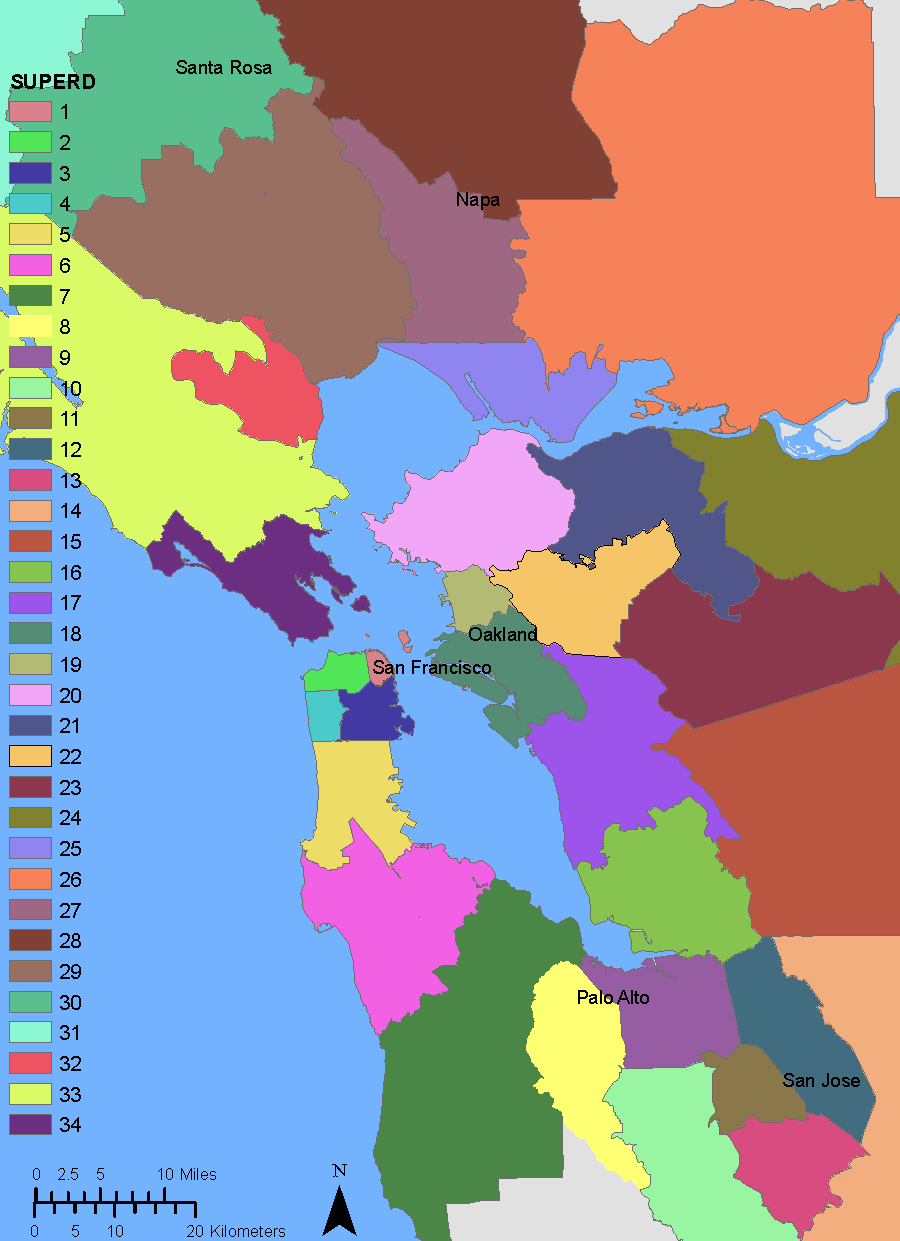
\includegraphics[width=5.5in]{FIGS/methods_super.pdf} 
%\caption{Map of 34 superdistricts.}
%\label{fig:superdistricts}
%\end{figure}
%
%\begin{figure}[ht]
%\centering
%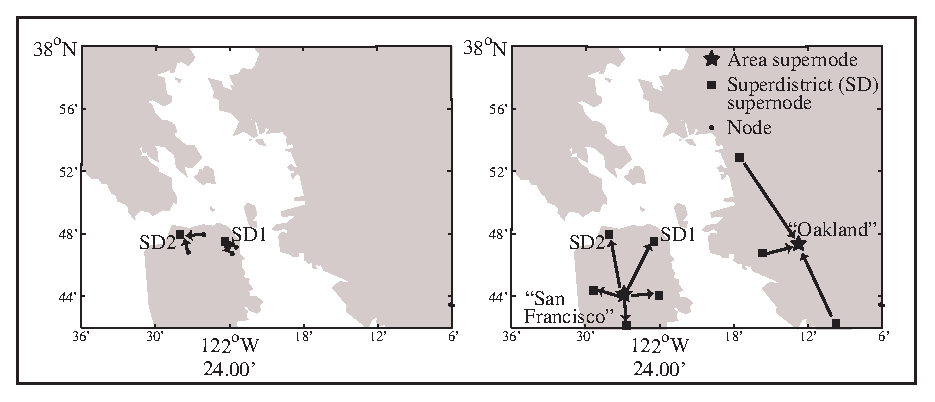
\includegraphics[width=6in]{FIGS/methods_superNode.eps} 
%\caption{Map of supernodes for a) local flow between superdistrict one (SD1) \emph{supernode} and superdistrict two (SD2)  \emph{supernode}, and b) San Francisco \emph{area supernode} to Oakland  \emph{area supernode}. Some nodes, representing road intersections, in the road graph G connect to or from superdistrict supernodes. Some superdistrict supernodes connect to or from area supernodes.}
%\label{fig:centroids}
%\end{figure}

%We compute the fixed-demand travel time by xxxx $$

\subsubsection{Event set selection using optimization}
From a large set of ground-motion intensity maps and damage maps, we choose a set of forty maps, using the optimization procedure we proposed in Miller and Baker 2014~\cite{miller_ground-motion_2014}; we chose the fixed-demand travel time delay as the proxy metric, because it is related to travel time delays expected in the high-fidelity model. We then use the high-fidelity model to predict the transportation network impacts of the forty pairs of ground-motion intensity and damage maps. The outcome is forty sets of results for the target performance metric, mode-destination accessibility. Each accessibility value has a corresponding annual rate of occurrence.
In the following sections, we first compare region-wide results, and then focus on particular characteristics of three communities (Figure~\ref{fig:equity_study_area} shows the study area and three communities). Finally, we discuss generalizable trends.